
\documentclass[10pt, conference, compsocconf]{IEEEtran}

\ifCLASSINFOpdf
  \usepackage[pdftex]{graphicx}
  % declare the path(s) where your graphic files are
  \graphicspath{{./images/}}
  % and their extensions so you won't have to specify these with
  % every instance of \includegraphics
  \DeclareGraphicsExtensions{.pdf,.jpeg,.png,.jpg}
\else
  % or other class option (dvipsone, dvipdf, if not using dvips). graphicx
  % will default to the driver specified in the system graphics.cfg if no
  % driver is specified.
  \usepackage[dvips]{graphicx}
  % declare the path(s) where your graphic files are
  \graphicspath{{./images/}}
  % and their extensions so you won't have to specify these with
  % every instance of \includegraphics
  \DeclareGraphicsExtensions{.eps}
\fi

% correct bad hyphenation here
\hyphenation{op-tical net-works semi-conduc-tor}


\begin{document}
%
% paper title
% can use linebreaks \\ within to get better formatting as desired
\title{Usage Management of Electronic Medical Records}


% author names and affiliations
% use a multiple column layout for up to two different
% affiliations
\author{\IEEEauthorblockN{Christopher C. Lamb, Pramod A. Jamkhedkar, Gregory L. Heileman, Ravi Kadaboina}
\IEEEauthorblockA{University of New Mexico\\
Department of Electrical and Computer Engineering\\
Albuquerque, NM 87131-0001 \\
\{cclamb, pramod54, heileman, ravik\}@ece.unm.edu}
}

% conference papers do not typically use \thanks and this command
% is locked out in conference mode. If really needed, such as for
% the acknowledgment of grants, issue a \IEEEoverridecommandlockouts
% after \documentclass

% for over three affiliations, or if they all won't fit within the width
% of the page, use this alternative format:
% 
%\author{\IEEEauthorblockN{Michael Shell\IEEEauthorrefmark{1},
%Homer Simpson\IEEEauthorrefmark{2},
%James Kirk\IEEEauthorrefmark{3}, 
%Montgomery Scott\IEEEauthorrefmark{3} and
%Eldon Tyrell\IEEEauthorrefmark{4}}
%\IEEEauthorblockA{\IEEEauthorrefmark{1}School of Electrical and Computer Engineering\\
%Georgia Institute of Technology,
%Atlanta, Georgia 30332--0250\\ Email: see http://www.michaelshell.org/contact.html}
%\IEEEauthorblockA{\IEEEauthorrefmark{2}Twentieth Century Fox, Springfield, USA\\
%Email: homer@thesimpsons.com}
%\IEEEauthorblockA{\IEEEauthorrefmark{3}Starfleet Academy, San Francisco, California 96678-2391\\
%Telephone: (800) 555--1212, Fax: (888) 555--1212}
%\IEEEauthorblockA{\IEEEauthorrefmark{4}Tyrell Inc., 123 Replicant Street, Los Angeles, California 90210--4321}}

% make the title area
\maketitle


\begin{abstract}
Electronic medical record management is under new scruitiny as private companies move into the market and government agencies actively address percieved health care distribution inequalities and inefficiencies.  Current systems are coarse-grained and provide consumers very little actual control over their data.  Herein, we propose an alternative system for managing the use of healthcare infomormation.  This system is more granular, allows for data mining and repackaging, and gives users more control over data while allowing said data to be distributed as much as needed.  In this paper, we outline the characteristics of such a system, present relavant background information and research leading to the system design, and cover two specific use scenarios supported by this system that are difficult to control using simpler access control strategies.
\end{abstract}

\begin{IEEEkeywords}
%component; formatting; style; styling;
usage management; electronic medical records

\end{IEEEkeywords}


% For peer review papers, you can put extra information on the cover
% page as needed:
% \ifCLASSOPTIONpeerreview
% \begin{center} \bfseries EDICS Category: 3-BBND \end{center}
% \fi
%
% For peerreview papers, this IEEEtran command inserts a page break and
% creates the second title. It will be ignored for other modes.
\IEEEpeerreviewmaketitle

\section{Introduction}
% no \IEEEPARstart
New healthcare legislation has spurred previously unknown levels of public and private investment into technologies supporting more efficient healthcare delivery \cite{website:recovery}.   An active area of examination is electronic health records.  Current systems, like Microsoft HealthVault and Google Health are a start in this area, but provide rudimentary control over health information, provide consumers with very little actual control of their information, and essentially demand proprietary lockin to these products because of the amount of effort involved with data transfer \cite{Evaluation:HealthInf:10}.

We propose an open, consumer-centric approach to health information storage and consumption centered around flexible and granular usage management policies.  User empowering systems in this area are needed to allow users control over the information that represents them, and would be in high demand if appropriately designed \cite{Emr:PyAmWaCr:04}.  We propose to address this need by bundling health information (either entire records or subsets of records) with traceable and aggregateable usage policies controlled by the users themselves.  Users would have the ability to make aspects of their records available to everyone from research institutions looking for historical information for studies, to specific healthcare providers who need specific information to support diagnoses.  Furthermore, institutions would be able to combine information from groups of users and determine dynamically via policy evaluation how that new set of data can be used in a way that complies with all included user policies.  If the combined dataset cannot be used, policies can be analyzed to determine the cause of the policy conflict.

We will propose, design, and demonstrate a system that supports granular management of the data elements of an electronic medical record.  This management will allow users to specify policies over the data itself rather than the entire record in question, providing control over information dissemination.  We will demonstrate this control in three distinct scenarios.  The first will include two distinct parties negotiating over access to specific information contained in a medical record.  If the parties can reach an agreement, the information consumer will be granted access to specific medical data, for an agreed-upon price.  The second demostrates a data broker combining a set of previously acquired medical record data into an aggregate set for research, if the licensure is in fact compliant between all selelected data elements.  Finally, the aggregated data set will be placed back into the market.

This kind of system, allowing users control over their data in ways fostering ease of dissemination, use and reuse, helps users receive better, more targed care, helps providers easly access required information, and allows this kind of data to be more easily examined and mined.  We use established system design principles, used in the develoment of internet-scale networks to create a open flexible system \cite{Al:04,BlCl:01,ClWrSoBr:02}.  We will standardize certain features, such as operational semantics and ontological domains, but otherwise limit the impact of the policy system on data dissemination as much as possible.

\subsection{Previous Work}
Past research applicable to this area includes usage management, digital rights management (DRM), and access control.  Most of the research applicable to the combination of previous arfifacts into a single aggregate artifact comes from the DRM world in particular.  Generally, these expressive languages have been fundamentally based on different types of mathematical logic or formalisms with reasoning capabilities \cite{ArHu:07,BaMi:06,ChCoEtHaJoLa:03,HaWe:04,HaWe:08,PuWe:02,XiBjFu:08}.  This approach, while useful in closed systems, tends to not work as usefully in more open dynamic environments.  This has led to the development of translation mechanisms to address interoperability needs \cite{HeJa:05,PoPrDe:04,ScTaWo:04}.  This translation process is difficult for most policy languages, and in fact infeasible as a result \cite{KoLaMaMi:04,SaShUe:04}.  Alternative approaches have required the use of sophiticated and powerful languages that must be adopted as a universal standard \cite{OMADRM,ODRL-req,Wa:04,XrML-spec}.  This approach inherently limits innovation and flexibility \cite{HeJa:05,JaHe:04,JaHe:08,JaHeMa:06}.

%\subsubsection{Subsubsection Heading Here}
%Subsubsection text here.

\section{Underpinnings}
%Wherever Times is specified, Times Roman or Times New Roman may be used. If neither is available on your system, please use the font closest in appearance to Times. Avoid using bit-mapped fonts if possible. True-Type 1 or Open Type fonts are preferred. Please embed symbol fonts, as well, for math, etc.
Describe details of technology including ontologies; need to discuss static v. dynamic term evaluation and why we require dynamic in this system 

\subsection{Marketplace}
describe how the market works, how it incentivises desired behaviour

\begin{figure}[!t]
\centering
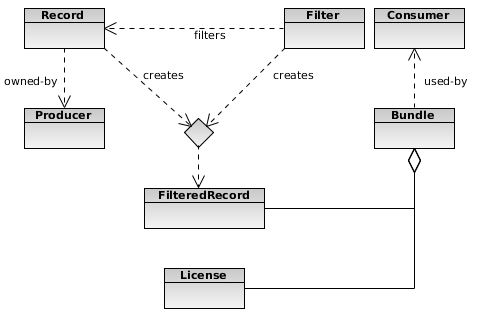
\includegraphics[width=3in]{ontology}
\caption{Simulation Results}
\label{fig_sim}
\end{figure}

\subsection{Usage Management}
describe how the usage management system works

\section{System}
%Wherever Times is specified, Times Roman or Times New Roman may be used. If neither is available on your system, please use the font closest in appearance to Times. Avoid using bit-mapped fonts if possible. True-Type 1 or Open Type fonts are preferred. Please embed symbol fonts, as well, for math, etc.

\subsection{Cases and Scenarios}
Outline the use cases, describe them, map them to specific scenarios

\subsection{Scenario 1: Negotiation}
Demonstrate and present results; negotiation over specific information contained in a EMR

\subsection{Scenario 2: Aggregate Assembly}
Demonstrate and present results; assemble data elements into a single data set; show both usage term compliance and non-compliance

\subsection{Scenario 3: Aggregate Submission}
Demonstrate and present results; insert new set into marketplace; demonstrate acquisition of set and traceability back to individual elements

% An example of a floating figure using the graphicx package.
% Note that \label must occur AFTER (or within) \caption.
% For figures, \caption should occur after the \includegraphics.
% Note that IEEEtran v1.7 and later has special internal code that
% is designed to preserve the operation of \label within \caption
% even when the captionsoff option is in effect. However, because
% of issues like this, it may be the safest practice to put all your
% \label just after \caption rather than within \caption{}.
%
% Reminder: the "draftcls" or "draftclsnofoot", not "draft", class
% option should be used if it is desired that the figures are to be
% displayed while in draft mode.
%
%\begin{figure}[!t]
%\centering
%\includegraphics[width=2.5in]{myfigure}
% where an .eps filename suffix will be assumed under latex, 
% and a .pdf suffix will be assumed for pdflatex; or what has been declared
% via \DeclareGraphicsExtensions.
%\caption{Simulation Results}
%\label{fig_sim}
%\end{figure}

% Note that IEEE typically puts floats only at the top, even when this
% results in a large percentage of a column being occupied by floats.


% An example of a double column floating figure using two subfigures.
% (The subfig.sty package must be loaded for this to work.)
% The subfigure \label commands are set within each subfloat command, the
% \label for the overall figure must come after \caption.
% \hfil must be used as a separator to get equal spacing.
% The subfigure.sty package works much the same way, except \subfigure is
% used instead of \subfloat.
%
%\begin{figure*}[!t]
%\centerline{\subfloat[Case I]\includegraphics[width=2.5in]{subfigcase1}%
%\label{fig_first_case}}
%\hfil
%\subfloat[Case II]{\includegraphics[width=2.5in]{subfigcase2}%
%\label{fig_second_case}}}
%\caption{Simulation results}
%\label{fig_sim}
%\end{figure*}
%
% Note that often IEEE papers with subfigures do not employ subfigure
% captions (using the optional argument to \subfloat), but instead will
% reference/describe all of them (a), (b), etc., within the main caption.


% An example of a floating table. Note that, for IEEE style tables, the 
% \caption command should come BEFORE the table. Table text will default to
% \footnotesize as IEEE normally uses this smaller font for tables.
% The \label must come after \caption as always.
%
%\begin{table}[!t]
%% increase table row spacing, adjust to taste
%\renewcommand{\arraystretch}{1.3}
% if using array.sty, it might be a good idea to tweak the value of
% \extrarowheight as needed to properly center the text within the cells
%\caption{An Example of a Table}
%\label{table_example}
%\centering
%% Some packages, such as MDW tools, offer better commands for making tables
%% than the plain LaTeX2e tabular which is used here.
%\begin{tabular}{|c||c|}
%\hline
%One & Two\\
%\hline
%Three & Four\\
%\hline
%\end{tabular}
%\end{table}


% Note that IEEE does not put floats in the very first column - or typically
% anywhere on the first page for that matter. Also, in-text middle ("here")
% positioning is not used. Most IEEE journals/conferences use top floats
% exclusively. Note that, LaTeX2e, unlike IEEE journals/conferences, places
% footnotes above bottom floats. This can be corrected via the \fnbelowfloat
% command of the stfloats package.



\section{Conclusion}
Evaluate results and outline future work

% conference papers do not normally have an appendix


% use section* for acknowledgement
\section*{Acknowledgment}
The authors would like to thank ECE, Ravi, Greg, Pramod?


% trigger a \newpage just before the given reference
% number - used to balance the columns on the last page
% adjust value as needed - may need to be readjusted if
% the document is modified later
%\IEEEtriggeratref{8}
% The "triggered" command can be changed if desired:
%\IEEEtriggercmd{\enlargethispage{-5in}}

% references section

% can use a bibliography generated by BibTeX as a .bbl file
% BibTeX documentation can be easily obtained at:
% http://www.ctan.org/tex-archive/biblio/bibtex/contrib/doc/
% The IEEEtran BibTeX style support page is at:
% http://www.michaelshell.org/tex/ieeetran/bibtex/
%\bibliographystyle{IEEEtran}
% argument is your BibTeX string definitions and bibliography database(s)
%\bibliography{IEEEabrv,../bib/paper}
%
% <OR> manually copy in the resultant .bbl file
% set second argument of \begin to the number of references
% (used to reserve space for the reference number labels box)
%\begin{thebibliography}{1}
\bibliographystyle{plain}
\bibliography{emr,drm}

%\bibitem{IEEEhowto:kopka}
%H.~Kopka and P.~W. Daly, \emph{A Guide to \LaTeX}, 3rd~ed.\hskip 1em plus
%  0.5em minus 0.4em\relax Harlow, England: Addison-Wesley, 1999.
  
%\bibitem{Jamkhedkar:Heileman}
%P.A.~Jamkhedkar and G.~L. Heileman, \emph{An Interoperable Usage Management Framework},
%  ACM DRM 2010, Chicago Ill, USA, 2010.

%\end{thebibliography}




% that's all folks
\end{document}


